% \qrchapter{https://forgottenpillar.com/rsc/en-fp-chapter14}{Adventist pioneers and the Trinity doctrine}


\qrchapter{https://forgottenpillar.com/rsc/ro-fp-chapter14}{Pionierii adventiști și doctrina Trinității}


Sister White wrote that early Adventist pioneers \egwinline{are to bear their testimony as to what constitutes the truth for this time}[Lt329-1905.18; 1905][https://egwwritings.org/read?panels=p8455.24] because \egwinline{they have learned to avoid errors and dangers, and are they not then competent to give wise counsel}[7T 287.3; 1902][https://egwwritings.org/read?panels=p117.1637]? In their writings, we see their unanimous views regarding the \emcap{personality of God}, and that they have avoided the Trinitarian error. There is much to write about this topic because the Adventist pioneers left a lot of material dealing directly or indirectly with the doctrine of Trinity. But we will look at some of the testimonies from James White and brother Loughborough because we have read some of their articles on the \emcap{personality of God}. Also, we will compare their testimony with the Spirit of Prophecy as we have done so far.


Sora White a scris că pionierii adventiști timpurii \egwinline{trebuie să-și aducă mărturia cu privire la ceea ce constituie adevărul pentru acest timp}[Lt329-1905.18; 1905][https://egwwritings.org/read?panels=p8455.24] deoarece \egwinline{ei au învățat să evite erorile și pericolele, și nu sunt ei atunci competenți să dea sfaturi înțelepte}[7T 287.3; 1902][https://egwwritings.org/read?panels=p117.1637]? În scrierile lor, vedem părerile lor unanime cu privire la \emcap{personalitatea lui Dumnezeu}, și că au evitat eroarea trinitariană. Există mult de scris despre acest subiect deoarece pionierii adventiști au lăsat mult material care tratează direct sau indirect doctrina Trinității. Dar vom privi la câteva dintre mărturiile lui James White și ale fratelui Loughborough deoarece am citit câteva dintre articolele lor despre \emcap{personalitatea lui Dumnezeu}. De asemenea, vom compara mărturia lor cu Spiritul Profetic așa cum am făcut până acum.


James White, in the Review and Herald, listed \others{some of \textbf{the popular fables} of the age}”, saying: “\others{Here we might mention \textbf{the Trinity, which \underline{does away the personality of God, and of his Son Jesus Christ,} }and of sprinkling or pouring instead of being ‘buried with Christ in baptism,’ ‘planted in the likeness of his death:’ but we pass from these \textbf{fables }to notice one that is held sacred by nearly all professed Christians, both Catholic and Protestant. It is, the change of the Sabbath of the fourth commandment from the seventh to the first day of the week.}[James S. White, Review \& Herald, December 11, 1855, p. 85.15][http://documents.adventistarchives.org/Periodicals/RH/RH18551211-V07-11.pdf]


James White, în Review and Herald, a enumerat \others{câteva dintre \textbf{fabulele populare} ale epocii}, spunând: „\others{Aici am putea menționa \textbf{Trinitatea, care \underline{desființează personalitatea lui Dumnezeu și a Fiului Său Isus Hristos,} }și stropirea sau turnarea în loc de a fi ‘îngropați cu Hristos în botez’, ‘sădiți în asemănarea morții Lui’: dar trecem de la aceste \textbf{fabule }pentru a observa una care este considerată sacră de aproape toți creștinii mărturisiți, atât catolici cât și protestanți. Este schimbarea Sabatului poruncii a patra de la ziua a șaptea la prima zi a săptămânii.}[James S. White, Review \& Herald, December 11, 1855, p. 85.15][http://documents.adventistarchives.org/Periodicals/RH/RH18551211-V07-11.pdf]


What does James White mean when he says that the Trinity \others{does away with the personality of God, and of his Son Jesus Christ}? In Day Star, he wrote:


Ce vrea să spună James White când spune că Trinitatea \others{desființează personalitatea lui Dumnezeu și a Fiului Său Isus Hristos}? În Day Star, el a scris:


\others{…a certain class who \textbf{deny the only Lord God and our Lord Jesus Christ}. This class can be no other than those who \textbf{spiritualize away the existence of the Father and the Son}, \textbf{as \underline{two distinct}, \underline{literal}, \underline{tangible persons}}, also a literal Holy city and throne of David… The way spiritualizers this way have disposed of or \textbf{denied the only Lord God and our Lord Jesus Christ is first using \underline{the old unscriptural trinitarian creed}}, viz, that Jesus Christ is the eternal God, though they have not one passage to support it, while we have plain scripture testimony in abundance \textbf{that He is the Son of the eternal God.}}[James White, Day Star, Jan 24, 1846][https://m.egwwritings.org/en/book/741.25\#27]


\others{...o anumită clasă care \textbf{neagă pe singurul Domn Dumnezeu și pe Domnul nostru Isus Hristos}. Această clasă nu poate fi alta decât cei care \textbf{spiritualizează existența Tatălui și a Fiului}, \textbf{ca \underline{două persoane distincte}, \underline{literale}, \underline{tangibile}}, de asemenea o cetate sfântă literală și tronul lui David... Modul în care cei care spiritualizează au înlăturat sau \textbf{au negat pe singurul Domn Dumnezeu și pe Domnul nostru Isus Hristos este mai întâi folosind \underline{vechiul crez trinitarian nescriptural}}, adică, că Isus Hristos este Dumnezeul etern, deși ei nu au niciun pasaj care să-l susțină, în timp ce noi avem mărturie scripturală clară din abundență \textbf{că El este Fiul Dumnezeului etern.}}[James White, Day Star, Jan 24, 1846][https://m.egwwritings.org/en/book/741.25\#27]


Doing away with the personality of God and His Son is accomplished by denying Them as two distinct, literal, and tangible persons. The doctrine on the personality of God teaches that the Father has a literal, \textit{tangible} person.


Desființarea personalității lui Dumnezeu și a Fiului Său se realizează prin negarea Lor ca două persoane distincte, literale și tangibile. Doctrina despre personalitatea lui Dumnezeu învață că Tatăl are o persoană literală, \textit{tangibilă}.


In the Adventist Review and Sabbath Herald article from April 4, 1854, James White listed 10 points of \textit{Catholic reasons for keeping Sunday}”, where he said that the Sunday \others{is a day dedicated by the apostles to \textbf{the honor of the most Holy Trinity}}[The Advent Review, and Sabbath Herald, vol. 5 April 4, 1854, p. 86][https://egwwritings.org/read?panels=p1643.2867]. Here we also see the harmony between J. B. Frisbie and James White in their view that the Sabbath is dedicated to the biblical God expressed in the first point of the \emcap{Fundamental Principles}, and Sunday is dedicated to the trinity God. The main problem with the Trinity doctrine is that it \others{does away the personality of God, and of his Son Jesus Christ}. In Life Incidents, he wrote more about why this is so.


În articolul din Adventist Review and Sabbath Herald din 4 aprilie 1854, James White a enumerat 10 puncte ale \textit{motivelor catolice pentru păzirea duminicii}”, unde a spus că duminica \others{este o zi dedicată de apostoli \textbf{onoarei preasfintei Trinități}}[The Advent Review, and Sabbath Herald, vol. 5 April 4, 1854, p. 86][https://egwwritings.org/read?panels=p1643.2867]. Aici vedem de asemenea armonia dintre J. B. Frisbie și James White în viziunea lor că Sabatul este dedicat Dumnezeului biblic exprimat în primul punct al \emcap{Principiilor Fundamentale}, iar duminica este dedicată Dumnezeului trinitar. Problema principală cu doctrina Trinității este că \others{desființează personalitatea lui Dumnezeu și a Fiului Său Isus Hristos}. În Life Incidents, el a scris mai mult despre de ce este așa.


\others{\textbf{Jesus prayed that his disciples might be one as he was \underline{one with his Father}}. \textbf{This prayer did not contemplate one disciple with twelve heads, but twelve disciples, made one in object and effort in the cause of their Master}. \textbf{\underline{Neither are the Father and the Son parts of the ‘three-one God.}}’\footnote{The same quotation is found in James White’s book “\textit{The Law and the Gospel}” with one difference. He states, “\textit{Neither are the Father and the Son parts of \underline{one being}}”; in “\textit{Life Incidents}”, he wrote “parts of the ‘\underline{three-one God}’”. See \href{https://egwwritings.org/?ref=en_LAGO.1.2&para=1492.10}{James S. White, The Law and the Gospel p. 1.2}.} \textbf{\underline{They are two distinct beings}}, \textbf{yet one in the design and accomplishment of redemption}. The redeemed, from the first who shares in the great redemption, to the last, all ascribe the honour, and glory, and praise, of their salvation, to \textbf{both God and the Lamb}.}[James S. White, Life Incidents, p.343.2][https://egwwritings.org/read?panels=p1462.1743]


\others{\textbf{Isus s-a rugat ca ucenicii Săi să fie una așa cum El era \underline{una cu Tatăl Său}}. \textbf{Această rugăciune nu a avut în vedere un ucenic cu doisprezece capete, ci doisprezece ucenici, făcuți una în obiectiv și efort în cauza Stăpânului lor}. \textbf{\underline{Nici Tatăl și Fiul nu sunt părți ale ‘Dumnezeului trei-în-unul.}}’\footnote{Același citat se găsește în cartea lui James White „\textit{The Law and the Gospel}” cu o diferență. El afirmă, „\textit{Nici Tatăl și Fiul nu sunt părți ale \underline{unei singure ființe}}”; în „\textit{Life Incidents}”, el a scris „părți ale ‘\underline{Dumnezeului trei-în-unul}’“. Vezi \href{https://egwwritings.org/?ref=en_LAGO.1.2&para=1492.10}{James S. White, The Law and the Gospel p. 1.2}.} \textbf{\underline{Ei sunt două ființe distincte}}, \textbf{totuși una în planul și împlinirea răscumpărării}. Cei răscumpărați, de la primul care are parte de marea răscumpărare, până la ultimul, toți atribuie onoarea, gloria și lauda salvării lor, atât \textbf{lui Dumnezeu cât și Mielului}.}[James S. White, Life Incidents, p.343.2][https://egwwritings.org/read?panels=p1462.1743]


Sister White wrote similarly regarding Christ’s prayer:


Sora White a scris în mod similar cu privire la rugăciunea lui Hristos:


\egw{The burden of that prayer was that His disciples might be \textbf{one as He was one with the Father}; the oneness so close that, \textbf{although \underline{two distinct beings}}, there was \textbf{perfect unity of spirit, purpose, and action}. The mind of the Father was the mind of the Son.}[Lt1-1882.1; 1882][https://egwwritings.org/read?panels=p4120.5]


\egw{Povara acelei rugăciuni era ca ucenicii Săi să fie \textbf{una așa cum El era una cu Tatăl}; unitatea atât de strânsă încât, \textbf{deși \underline{două ființe distincte}}, exista \textbf{unitate perfectă de spirit, scop și acțiune}. Mintea Tatălui era mintea Fiului.}[Lt1-1882.1; 1882][https://egwwritings.org/read?panels=p4120.5]


\egw{\textbf{The unity that exists between Christ and His disciples \underline{does not destroy the personality of either}}. They are one in purpose, in mind, in character, \textbf{but \underline{not in person}}. \textbf{It is thus that God and Christ are one}.}[MH, 421 422; 1905][https://egwwritings.org/read?panels=p135.2177]


\egw{\textbf{Unitatea care există între Hristos și ucenicii Săi \underline{nu distruge personalitatea niciunuia dintre ei}}. Ei sunt una în scop, în minte, în caracter, \textbf{dar \underline{nu în persoană}}. \textbf{Astfel sunt Dumnezeu și Hristos una}.}[MH, 421 422; 1905][https://egwwritings.org/read?panels=p135.2177]


The Father and the Son do not comprise one person nor being. The Father and the Son are one, just as Christ and His disciples are one—one in spirit, purpose, mind, and character.


Tatăl și Fiul nu alcătuiesc o singură persoană sau ființă. Tatăl și Fiul sunt una, așa cum Hristos și ucenicii Săi sunt una—una în spirit, scop, minte și caracter.


Many Adventist trinitarian scholars charge James White and other early pioneers for arianism or semi-arianism, claiming that they made Christ inferior to the Father. This is not true. Let us read the testimony of James White on this matter.


Mulți învățați adventiști trinitarieni îl acuză pe James White și pe alți pionieri timpurii de arianism sau semi-arianism, susținând că L-au făcut pe Hristos inferior Tatălui. Acest lucru nu este adevărat. Să citim mărturia lui James White în această privință.


\others{Paul affirms of \textbf{the Son of God that he was in the form of God}, and that \textbf{\underline{he was equal with God}}. ‘\textbf{Who being in the form of God thought it not robbery to be \underline{equal with God}}.’ Phil. 2:6. The reason why it is not robbery for the Son \textbf{to be equal with the Father is the fact that he is equal}. If the Son is not equal with the Father, then it is robbery for him to rank himself with the Father.}


\others{Pavel afirmă despre \textbf{Fiul lui Dumnezeu că era în chipul lui Dumnezeu}, și că \textbf{\underline{era egal cu Dumnezeu}}. ‘\textbf{El, măcar că avea chipul lui Dumnezeu, totuși n-a crezut ca un lucru de apucat să fie \underline{deopotrivă cu Dumnezeu}}.’ Filipeni 2:6. Motivul pentru care nu este o uzurpare ca Fiul \textbf{să fie egal cu Tatăl este faptul că el este egal}. Dacă Fiul nu este egal cu Tatăl, atunci este o uzurpare pentru el să se situeze la același rang cu Tatăl.}


\othersnogap{\textbf{\underline{The inexplicable trinity that makes the godhead three in one and one in three, is bad enough}}; \textbf{but that ultra Unitarianism that makes Christ inferior to the Father is worse}. Did God say to an inferior, Let us make man in our image?’}[James S. White, The Advent Review and Sabbath Herald, November 29, 1877, p. 171][https://documents.adventistarchives.org/Periodicals/RH/RH18771129-V50-22.pdf]


\othersnogap{\textbf{\underline{Trinitatea inexplicabilă care face ca dumnezeirea să fie trei în unul și unul în trei, este destul de rea}}; \textbf{dar acel unitarianism extrem care Îl face pe Hristos inferior Tatălui este mai rău}. A spus oare Dumnezeu unui inferior: Să facem om după chipul Nostru?’}[James S. White, The Advent Review and Sabbath Herald, November 29, 1877, p. 171][https://documents.adventistarchives.org/Periodicals/RH/RH18771129-V50-22.pdf]


The problem of the Adventist trinitarian scholars lies in that they themselves cannot completely explain Christ’s divinity other than through the Trinitarian paradigm. Adventist pioneers did believe in Christ’s full divinity but they rejected the Trinity because it destroys the \emcap{personality of God}. \others{The inexplicable trinity that makes the godhead three in one and one in three, \textbf{is bad enough}}. Below is another statement from James White where he compared Seventh-day Adventist with Seventh-day Baptist belief. Seventh-day Adventists did not believe in the Trinity unlike Seventh-day Baptists. James White mentioned that, regarding the divinity of Christ, Seventh-day Adventists hold so nearly with the trinitarian Seventh-day Baptists that they apprehend no trial there.


Problema învățaților adventiști trinitarieni constă în faptul că ei înșiși nu pot explica complet divinitatea lui Hristos altfel decât prin paradigma trinitariană. Pionierii adventiști au crezut într-adevăr în divinitatea deplină a lui Hristos, dar au respins Trinitatea pentru că aceasta distruge \emcap{personalitatea lui Dumnezeu}. \others{Trinitatea inexplicabilă care face ca dumnezeirea să fie trei în unul și unul în trei, \textbf{este destul de rea}}. Mai jos este o altă declarație de la James White unde a comparat credința adventiștilor de ziua a șaptea cu cea a baptiștilor de ziua a șaptea. Adventiștii de ziua a șaptea nu credeau în Trinitate, spre deosebire de baptiștii de ziua a șaptea. James White a menționat că, în privința divinității lui Hristos, adventiștii de ziua a șaptea susțin atât de aproape cu baptiștii trinitarieni de ziua a șaptea încât nu anticipează nicio dificultate acolo.


\others{\textbf{The principal difference between the two bodies is the immortality question}. \textbf{The S. D. Adventists hold \underline{the divinity of Christ so nearly with the trinitarian}, that we apprehend no trial here}. And as the practical application of the subject of the Gifts of the Spirit to our people and to our work is better understood by our S. D. Baptist brethren, they manifest less concern for us on this account.}[James S. White, The Advent Review and Sabbath Herald, October 12, 1876, p. 116][https://documents.adventistarchives.org/Periodicals/RH/RH18761012-V48-15.pdf]


\others{\textbf{Principala diferență dintre cele două grupuri este chestiunea nemuririi}. \textbf{Adventiștii de ziua a șaptea susțin \underline{divinitatea lui Hristos atât de aproape cu trinitarienii}, încât nu anticipăm nicio dificultate aici}. Și întrucât aplicarea practică a subiectului Darurilor Spirituale pentru poporul nostru și pentru lucrarea noastră este mai bine înțeleasă de frații noștri baptiști de ziua a șaptea, ei manifestă mai puțină îngrijorare pentru noi din acest motiv.}[James S. White, The Advent Review and Sabbath Herald, October 12, 1876, p. 116][https://documents.adventistarchives.org/Periodicals/RH/RH18761012-V48-15.pdf]


This evidence should raise questions to each Adventist trinitarian scholar. How could it be that the Adventist pioneers adhere to the divinity of Christ as trinitarians did, yet rejected the Trinity doctrine? In which way was Christ fully divine, if He was not part of an amalgamated three-in-one God? The answer is simple and completely Biblical. Christ is fully divine, just as His Father, because He was begotten in the express image of the Father’s person; thus, He inherited complete divine nature from His Father.


Această dovadă ar trebui să ridice întrebări fiecărui învățat adventist trinitarian. Cum se face că pionierii adventiști au aderat la divinitatea lui Hristos așa cum au făcut-o trinitarienii, și totuși au respins doctrina Trinității? În ce fel era Hristos pe deplin divin, dacă nu făcea parte dintr-un Dumnezeu amalgamat trei-în-unul? Răspunsul este simplu și complet biblic. Hristos este pe deplin divin, la fel ca Tatăl Său, pentru că a fost născut în întipărirea persoanei Tatălui; astfel, El a moștenit natura divină completă de la Tatăl Său.


\egw{A complete offering has been made; for ‘God so loved the world, that he gave his only-begotten Son,’—\textbf{not a son by creation}, as were the angels, nor a son by adoption, as is the forgiven sinner, but \textbf{a Son \underline{begotten} in the express image of the Father’s person}, and in all the brightness of his majesty and glory, \textbf{one equal with God} in authority, dignity, and \textbf{divine perfection}. \textbf{In him dwelt all the fullness of the Godhead bodily}.}[ST May 30, 1895, par. 3; 1895][https://egwwritings.org/read?panels=p820.12891]


\egw{O jertfă completă a fost făcută; căci ‘Fiindcă atât de mult a iubit Dumnezeu lumea, că a dat pe singurul Lui Fiu născut,’—\textbf{nu un fiu prin creație}, cum erau îngerii, nici un fiu prin adopție, cum este păcătosul iertat, ci \textbf{un Fiu \underline{născut} în întipărirea persoanei Tatălui}, și în toată strălucirea maiestății și gloriei Sale, \textbf{unul egal cu Dumnezeu} în autoritate, demnitate și \textbf{perfecțiune divină}. \textbf{În El locuiește toată plinătatea Dumnezeirii trupește}.}[ST May 30, 1895, par. 3; 1895][https://egwwritings.org/read?panels=p820.12891]


Christ's complete divinity is not based on an amalgamated \emcap{personality of God}, but rather on His Sonship with the Father. The Bible never refers to Christ with the term “\textit{one God}”—only the Father is referred to with the term “\textit{one God}”\footnote{John 17:3; 1. Corinthians 8:6; 1. Timothy 2:5; Ephesians 4:6} \footnote{We study Christ’s complete divinity in-depth  in the second book of the Forgotten Pillar Project - “\textit{Rediscovering the Pillar}”}. Jesus, the Son of God, is fully divine but is not referred to as \others{\textbf{one God}, \textbf{a personal, spiritual being}} in the first point of the \emcap{Fundamental Principles}.


Divinitatea completă a lui Hristos nu se bazează pe o \emcap{personalitate a lui Dumnezeu} amalgamată, ci mai degrabă pe Filiația Sa cu Tatăl. Biblia nu se referă niciodată la Hristos cu termenul “\textit{un singur Dumnezeu}”—doar Tatăl este menționat cu termenul “\textit{un singur Dumnezeu}”\footnote{Ioan 17:3; 1 Corinteni 8:6; 1 Timotei 2:5; Efeseni 4:6} \footnote{Studiem divinitatea completă a lui Hristos în profunzime în a doua carte a Proiectului Stâlpul Uitat - “\textit{Redescoperind Stâlpul}”}. Isus, Fiul lui Dumnezeu, este pe deplin divin, dar nu este menționat ca \others{\textbf{un singur Dumnezeu}, \textbf{o ființă personală, spirituală}} în primul punct al \emcap{Principiilor Fundamentale}.


\egw{The Lord Jesus Christ, the only begotten Son of the Father, \textbf{is truly God in infinity, \underline{but not in personality}}.}[Ms116-1905.19; 1905][https://egwwritings.org/read?panels=p10633.25]


\egw{Domnul Isus Hristos, singurul Fiu născut al Tatălui, \textbf{este cu adevărat Dumnezeu în infinitate, \underline{dar nu în personalitate}}.}[Ms116-1905.19; 1905][https://egwwritings.org/read?panels=p10633.25]


Brother J. N. Loughborough was asked to answer the question, \others{What serious objection is there to the doctrine of the Trinity?}[The question was asked by Brother W. W. Giles and it was sent to James S. White, who forwarded the question to Brother John N. Loughborough.]. As we read his answer, let us try to understand some of the reasons why the early pioneers did not adhere to this doctrine.


Fratele J. N. Loughborough a fost rugat să răspundă la întrebarea, \others{Care este obiecția serioasă față de doctrina Trinității?}[Întrebarea a fost pusă de fratele W. W. Giles și a fost trimisă lui James S. White, care a transmis întrebarea fratelui John N. Loughborough.]. Pe măsură ce citim răspunsul său, să încercăm să înțelegem câteva dintre motivele pentru care pionierii timpurii nu au aderat la această doctrină.


\others{There are many objections which we might urge, but on account of our limited space we shall reduce them to the three following: \textbf{1. It is contrary to common sense. 2. It is contrary to scripture. 3. Its origin is Pagan and fabulous.}}


\others{Există multe obiecții pe care le-am putea ridica, dar din cauza spațiului nostru limitat le vom reduce la următoarele trei: \textbf{1. Este contrară bunului simț. 2. Este contrară Scripturii. 3. Originea ei este păgână și fabuloasă.}}


\othersnogap{These positions we will remark upon briefly in their order. And 1. \textbf{It is not very consonant with common sense to talk of three being one, and one being three}. \textbf{Or as some express it, calling God ‘the Triune God,’ or ‘the three-one-God.’} \textbf{If Father, Son, and Holy Ghost are each God, it would be three Gods; for three times one is not one, but three}. \textbf{\underline{There is a sense in which they are one, but not one person, as claimed by Trinitarians}}}.


\othersnogap{Aceste poziții le vom comenta pe scurt în ordinea lor. Și 1. \textbf{Nu este foarte consonant cu bunul simț să vorbim despre trei fiind unul, și unul fiind trei}. \textbf{Sau cum exprimă unii, numind pe Dumnezeu „Dumnezeul Triun” sau „Dumnezeul trei-într-unul.”} \textbf{Dacă Tatăl, Fiul și Duhul Sfânt sunt fiecare Dumnezeu, ar fi trei Dumnezei; căci de trei ori unu nu este unu, ci trei}. \textbf{\underline{Există un sens în care ei sunt una, dar nu o singură persoană, așa cum pretind trinitarienii}}}.


\othersnogap{2. \textbf{It is contrary to Scripture}. \textbf{Almost any portion of the New Testament we may open which has occasion to speak of the Father and Son, represents them as two distinct persons}. \textbf{\underline{The seventeenth chapter of John is alone sufficient to refute the doctrine of the Trinity}}. \textbf{Over forty times in that one chapter Christ speaks of his Father as a person distinct from himself}. His Father was in heaven and he upon earth. The Father had sent him. Given to him those that believed. He was then to go to the Father.\textbf{ And in this very testimony he shows us in what consists the oneness of the Father and Son}.\textbf{\underline{ It is the same as the oneness of the members of Christ’s church}}. ‘\textbf{That \underline{they} all may be one; \underline{as} thou, Father, art in me, and I in thee, \underline{that they also} may be one in us}; that the world may believe that thou hast sent me. And the \textbf{glory which thou gavest me I have given them}; that \textbf{they may be one}, \textbf{even as we are one.}’ \textbf{Of one heart and one mind}. \textbf{Of one purpose} in all the plan devised for man’s salvation. \textbf{\underline{Read the seventeenth chapter of John, and see if it does not completely upset the doctrine of the Trinity}}.}


\othersnogap{2. \textbf{Este contrară Scripturii}. \textbf{Aproape orice porțiune din Noul Testament pe care o putem deschide care are ocazia să vorbească despre Tatăl și Fiul, îi reprezintă ca două persoane distincte}. \textbf{\underline{Capitolul al șaptesprezecelea din Ioan este singur suficient pentru a respinge doctrina Trinității}}. \textbf{De peste patruzeci de ori în acel singur capitol Hristos vorbește despre Tatăl Său ca o persoană distinctă de El însuși}. Tatăl Său era în cer și El pe pământ. Tatăl Îl trimisese. I-a dat pe cei care au crezut. El urma să meargă la Tatăl.\textbf{ Și în chiar această mărturie El ne arată în ce constă unitatea Tatălui și a Fiului}.\textbf{\underline{ Este aceeași cu unitatea membrilor bisericii lui Hristos}}. ‘\textbf{Ca \underline{toți} să fie una; \underline{precum} Tu, Tată, ești în Mine, și Eu în Tine, \underline{ca și ei} să fie una în Noi}; ca lumea să creadă că Tu M-ai trimis. Și \textbf{slava pe care Mi-ai dat-o, le-am dat-o lor}; ca \textbf{ei să fie una}, \textbf{precum și Noi suntem una.}’ \textbf{De o inimă și un gând}. \textbf{De un singur scop} în tot planul conceput pentru mântuirea omului. \textbf{\underline{Citiți capitolul al șaptesprezecelea din Ioan și vedeți dacă nu răstoarnă complet doctrina Trinității}}.}


\othersnogap{\textbf{To believe that doctrine, when reading the scripture we must believe that God sent himself into the world, died to reconcile the world to himself, raised himself from the dead, ascended to himself in heaven, pleads before himself in heaven to reconcile the world to himself, and is the only mediator between man and himself}. It will not do to substitute the human nature of Christ (according to Trinitarians) as the Mediator; for Clarke says, ‘Human blood can no more appease God than swine’s blood.’ Comment on 2 Samuel 21:10. \textbf{We must believe also that in the garden God prayed to himself, if it were possible, to let the cup pass from himself, and a thousand other \underline{such absurdities}}.}


\othersnogap{\textbf{Pentru a crede acea doctrină, când citim Scriptura trebuie să credem că Dumnezeu S-a trimis pe Sine însuși în lume, a murit pentru a reconcilia lumea cu Sine însuși, S-a înviat pe Sine însuși din morți, S-a înălțat la Sine însuși în cer, pledează înaintea Sa însuși în cer pentru a reconcilia lumea cu Sine însuși și este singurul mijlocitor între om și Sine însuși}. Nu va merge să substituim natura umană a lui Hristos (conform trinitarienilor) ca Mijlocitor; căci Clarke spune: „Sângele uman nu poate îmblânzi pe Dumnezeu mai mult decât sângele de porc.” Comentariu la 2 Samuel 21:10. \textbf{Trebuie să credem de asemenea că în grădină Dumnezeu S-a rugat Lui însuși, dacă ar fi posibil, să treacă paharul de la Sine însuși, și o mie de alte \underline{asemenea absurdități}}.}


\othersnogap{\textbf{Read carefully the following texts, comparing them with the idea that Christ is the Omnipotent, Omnipresent, Supreme, and only self-existent God: John 14:28; 17:3; 3:16; 5:19, 26; 11:15; 20:19; 8:50; 6:38; Mark 13:32; Luke 6:12; 22:69; 24:29; Matthew 3:17; 27:46; Galatians 3:20; 1 John 2:1; Revelation 5:7; Acts 17:31. Also see Matthew 11:25, 27; Luke 1:32; 22:42; John 3:35, 36; 5:19, 21, 22, 23, 25, 26; 6:40; 8:35, 36; 14:13; 1 Corinthians 15:28, etc}.}


\othersnogap{\textbf{Citiți cu atenție următoarele texte, comparându-le cu ideea că Hristos este Atotputernicul, Omniprezentul, Supremul și singurul Dumnezeu care există de la Sine: Ioan 14:28; 17:3; 3:16; 5:19, 26; 11:15; 20:19; 8:50; 6:38; Marcu 13:32; Luca 6:12; 22:69; 24:29; Matei 3:17; 27:46; Galateni 3:20; 1 Ioan 2:1; Apocalipsa 5:7; Faptele Apostolilor 17:31. De asemenea, vedeți Matei 11:25, 27; Luca 1:32; 22:42; Ioan 3:35, 36; 5:19, 21, 22, 23, 25, 26; 6:40; 8:35, 36; 14:13; 1 Corinteni 15:28, etc}.}


\othersnogap{\textbf{The word Trinity nowhere occurs in the Scriptures}. \textbf{The principal text supposed to teach it is 1 John 1:7\footnote{J. N. Loughborough made a typo in the original document, he wanted to point out to 1 John 5:7}, which is an interpolation}. Clarke says, ‘\textbf{Out of one hundred and thirteen manuscripts, the text is wanting in one hundred and twelve. It occurs in no MS. before the tenth century. And the first place the text occurs in Greek, is in the Greek translation of the acts of the Council of Lateran, held A. D. 1215}.’ - Comment. on John 1, and remarks at close of chap.}


\othersnogap{\textbf{Cuvântul Trinitate nu apare nicăieri în Scripturi}. \textbf{Textul principal presupus să o învețe este 1 Ioan 1:7\footnote{J. N. Loughborough a făcut o greșeală de tipar în documentul original, el a vrut să indice 1 Ioan 5:7}, care este o interpolare}. Clarke spune: ‘\textbf{Din o sută treisprezece manuscrise, textul lipsește în o sută doisprezece. Nu apare în niciun manuscris înainte de secolul al zecelea. Și primul loc unde textul apare în greacă este în traducerea grecească a actelor Conciliului de la Lateran, ținut în 1215 d.Hr.}’ - Comentariu la Ioan 1, și observații la sfârșitul capitolului.}


\othersnogap{3. \textbf{Its origin is pagan and fabulous}. Instead of pointing us to scripture for proof of the trinity, we are pointed to the trident of the Persians, with the assertion that by this they designed to teach the idea of a trinity, and if they had the doctrine of the trinity, they must have received it by tradition from the people of God. \textbf{But this is all assumed, for it is certain that the Jewish church held to no such doctrine. Says Mr. Summerbell, ‘A friend of mine who was present in a New York synagogue, asked the Rabbi for an explanation of the \underline{word ’elohim’}. A Trinitarian clergyman who stood by, replied, ‘Why, that has \underline{reference to the three persons in the Trinity},’ when a Jew stepped forward and said he must not mention that word again, or they would have to compel him to leave the house; \underline{for it was not permitted to mention the name of any strange god in the synagogue}.’}\footnote{Discussion between Summerbell and Flood on Trinity, p.38.} Milman says the idea of the Trident is fabulous. (Hist. Christianity, p.34.)}


\othersnogap{3. \textbf{Originea sa este păgână și fabuloasă}. În loc să ne îndrepte către Scriptură pentru dovada trinității, suntem îndreptați către tridentul perșilor, cu afirmația că prin aceasta ei au intenționat să învețe ideea unei trinități, și dacă ei au avut doctrina trinității, trebuie să o fi primit prin tradiție de la poporul lui Dumnezeu. \textbf{Dar toate acestea sunt presupuse, căci este cert că biserica iudaică nu a susținut o astfel de doctrină. Spune domnul Summerbell: „Un prieten de-al meu care era prezent într-o sinagogă din New York, l-a întrebat pe rabin pentru o explicație a \underline{cuvântului ‘elohim’}. Un cleric trinitarian care stătea alături a răspuns: „Păi, aceasta face \underline{referire la cele trei persoane din Trinitate}”, când un evreu a pășit înainte și a spus că nu trebuie să mai menționeze acel cuvânt din nou, sau vor fi nevoiți să-l oblige să părăsească casa; \underline{căci nu era permis să se menționeze numele vreunui dumnezeu străin în sinagogă}.’}\footnote{Discuție între Summerbell și Flood despre Trinitate, p.38.} Milman spune că ideea Tridentului este fabuloasă. (Ist. Creștinismului, p.34.)}


\othersnogap{\textbf{This doctrine of the trinity was brought into the church about the same time with image worship, and keeping the day of the sun, and is but Persian doctrine remodeled}. \textbf{It occupied about three hundred years from its introduction to bring the doctrine to what it is now. It was commenced about 325 A. D., and was not completed till 681.} See Milman’s Gibbon’s Rome, vol. iv, p.422. It was adopted in Spain in 589, in England in 596, in Africa in 534. - Gib. vol. iv, pp.114,345; Milner, vol. i, p.519.}[John N. Loughborough, The Adventist Review, and Sabbath Herald, November 5, 1861, p. 184][https://egwwritings.org/read?panels=p1685.6615]


\othersnogap{\textbf{Această doctrină a trinității a fost adusă în biserică cam în același timp cu închinarea la chipuri și păzirea zilei soarelui, și nu este decât doctrină persană remodelată}. \textbf{A ocupat aproximativ trei sute de ani de la introducerea sa pentru a aduce doctrina la ceea ce este acum. A fost începută în jurul anului 325 d.Hr. și nu a fost finalizată până în 681.} Vezi Milman's Gibbon's Rome, vol. iv, p.422. A fost adoptată în Spania în 589, în Anglia în 596, în Africa în 534. - Gib. vol. iv, pp.114,345; Milner, vol. i, p.519.}[John N. Loughborough, The Adventist Review, and Sabbath Herald, 5 noiembrie 1861, p. 184][https://egwwritings.org/read?panels=p1685.6615]


Brother Loughborough was the son of a Methodist minister and he was raised with the belief in the doctrine of Trinity. Besides the reasons he mentioned, he does not adhere to this doctrine because it is not in harmony with the truth on the \emcap{personality of God}. The seventeenth chapter of John is in harmony with the truth on the \emcap{personality of God} taught and practiced by the Seventh-day Adventists; the Trinity doctrine is not.


Fratele Loughborough era fiul unui pastor metodist și a fost crescut cu credința în doctrina Trinității. Pe lângă motivele pe care le-a menționat, el nu aderă la această doctrină pentru că nu este în armonie cu adevărul despre \emcap{personalitatea lui Dumnezeu}. Capitolul al șaptesprezecelea din Ioan este în armonie cu adevărul despre \emcap{personalitatea lui Dumnezeu} învățat și practicat de adventiștii de ziua a șaptea; doctrina Trinității nu este.


\begin{figure}[hp]
    \centering
    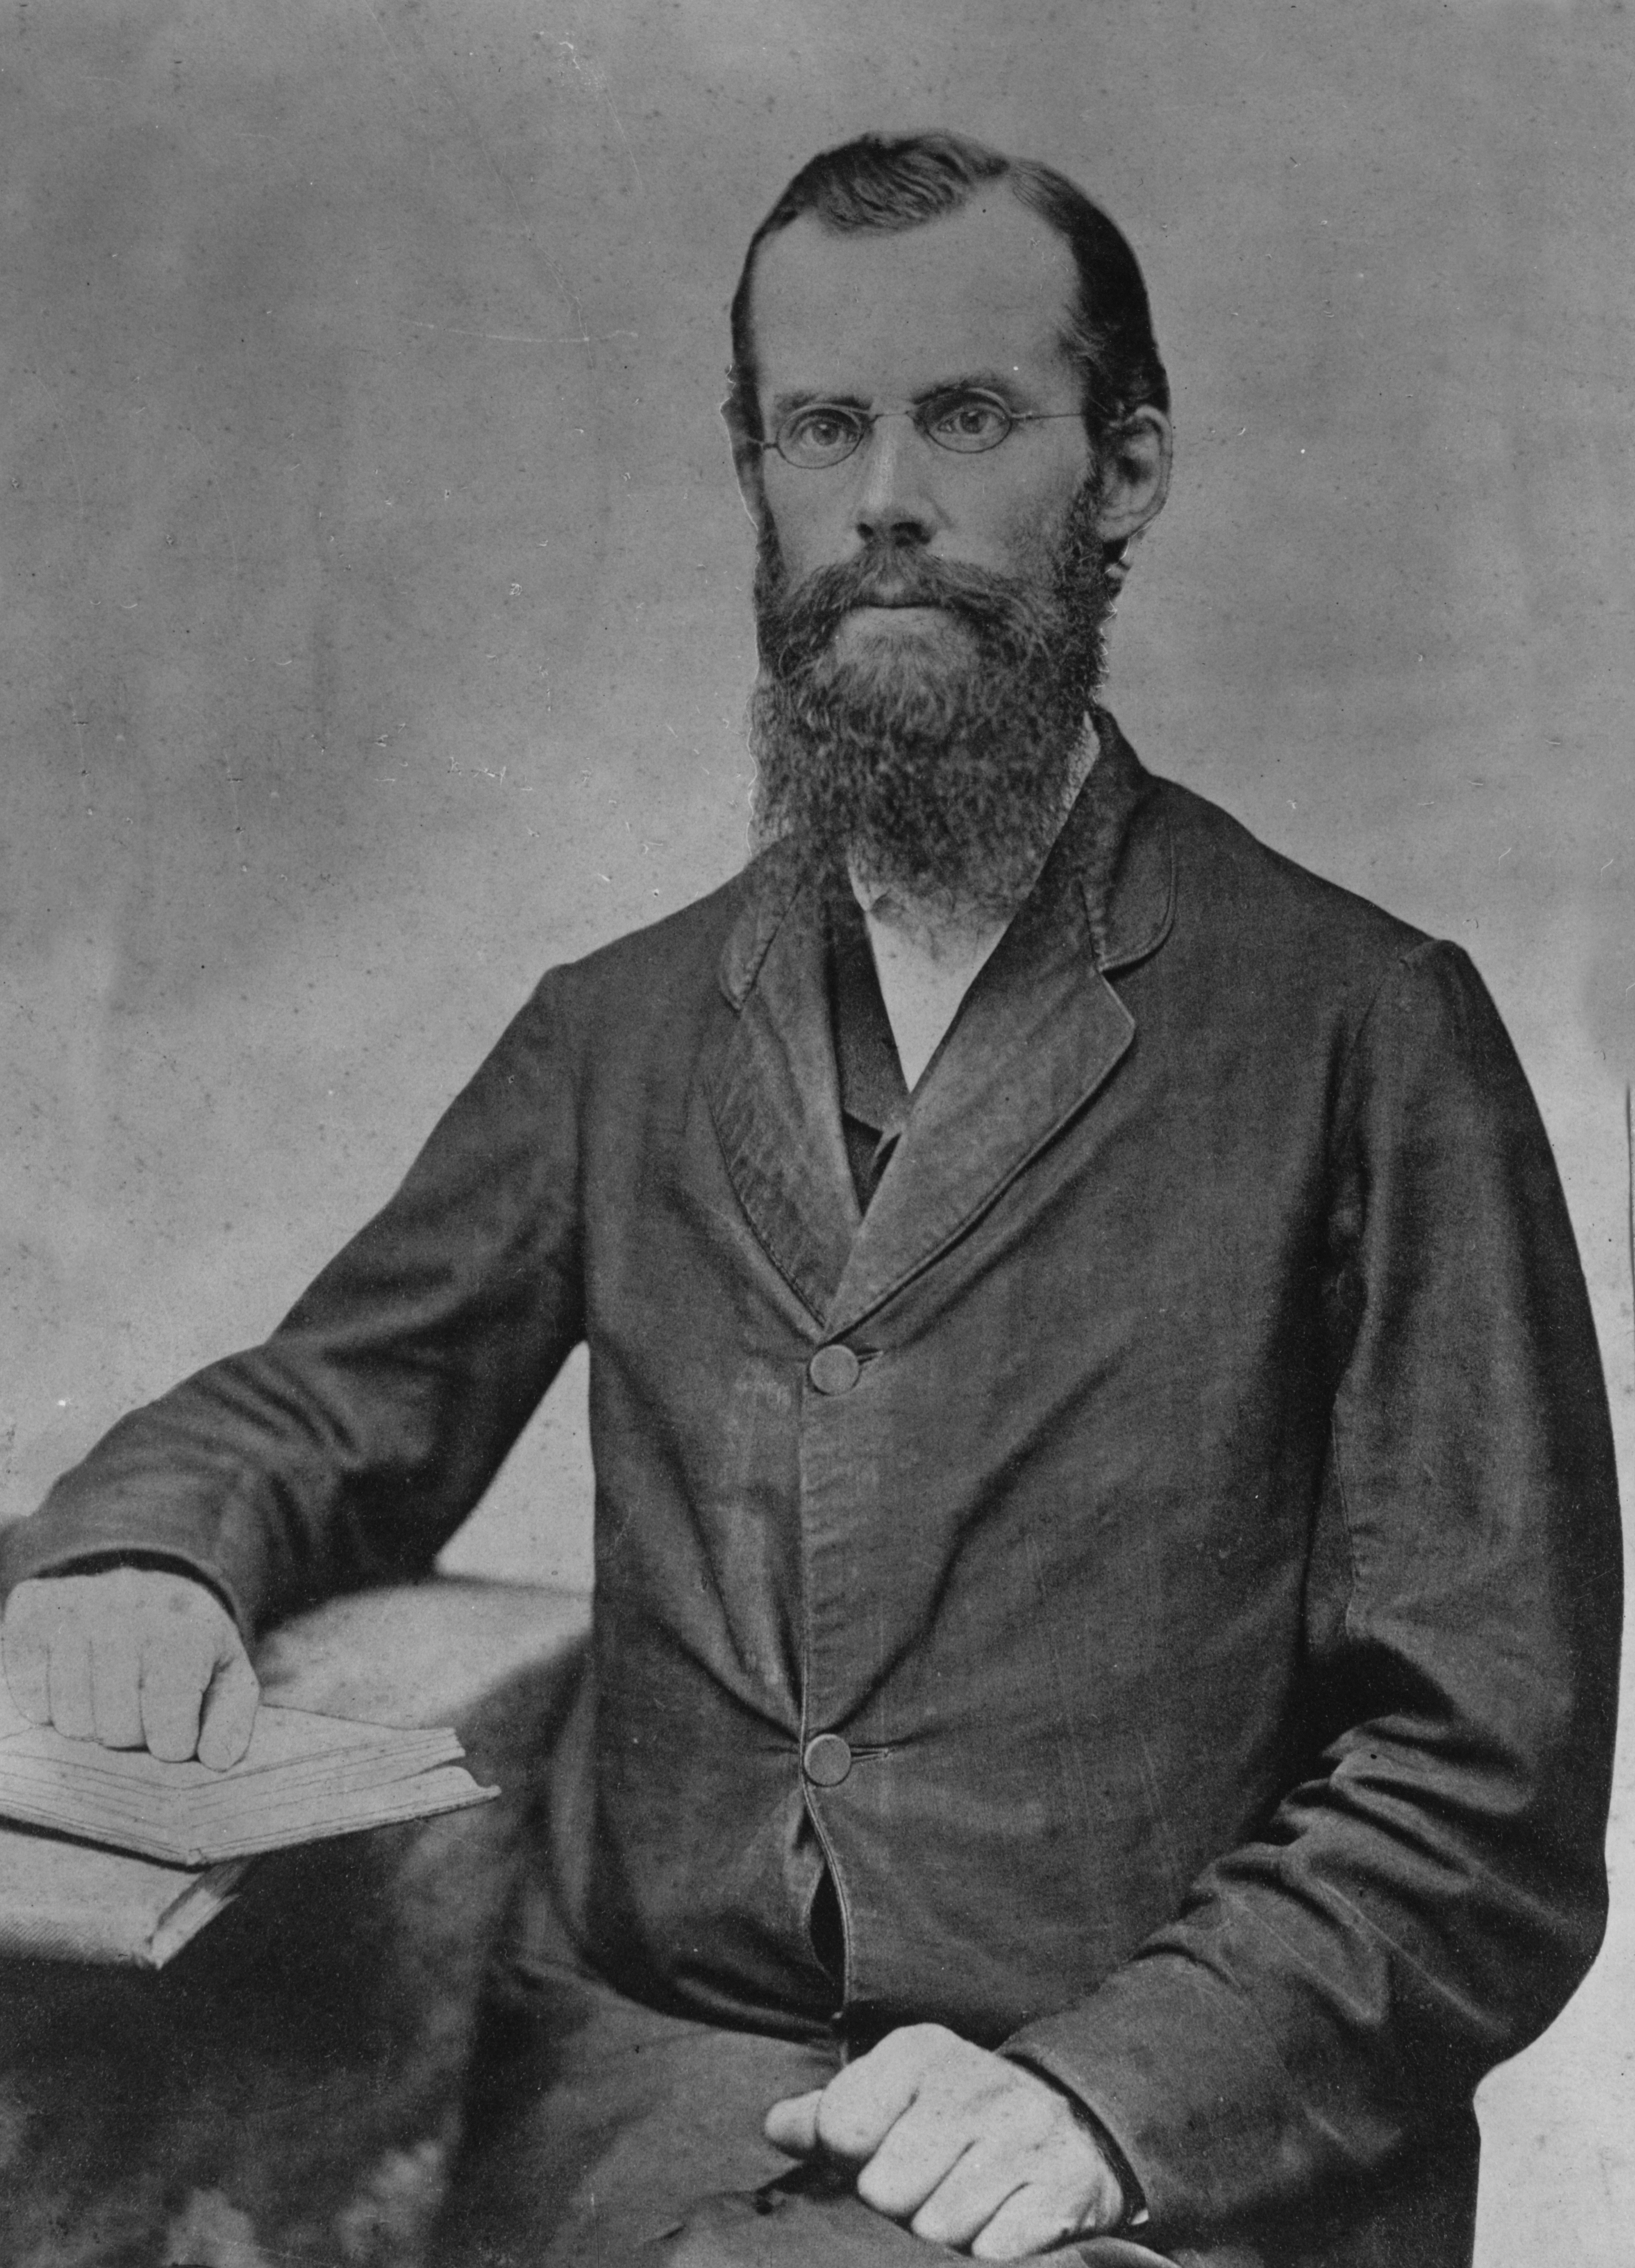
\includegraphics[width=1\linewidth]{images/john-nevins-andrews.jpg}
    \caption*{John Nevins Andrews (1829-1883)}
    \label{fig:j-n-andrews}
\end{figure}


\begin{figure}[hp]
    \centering
    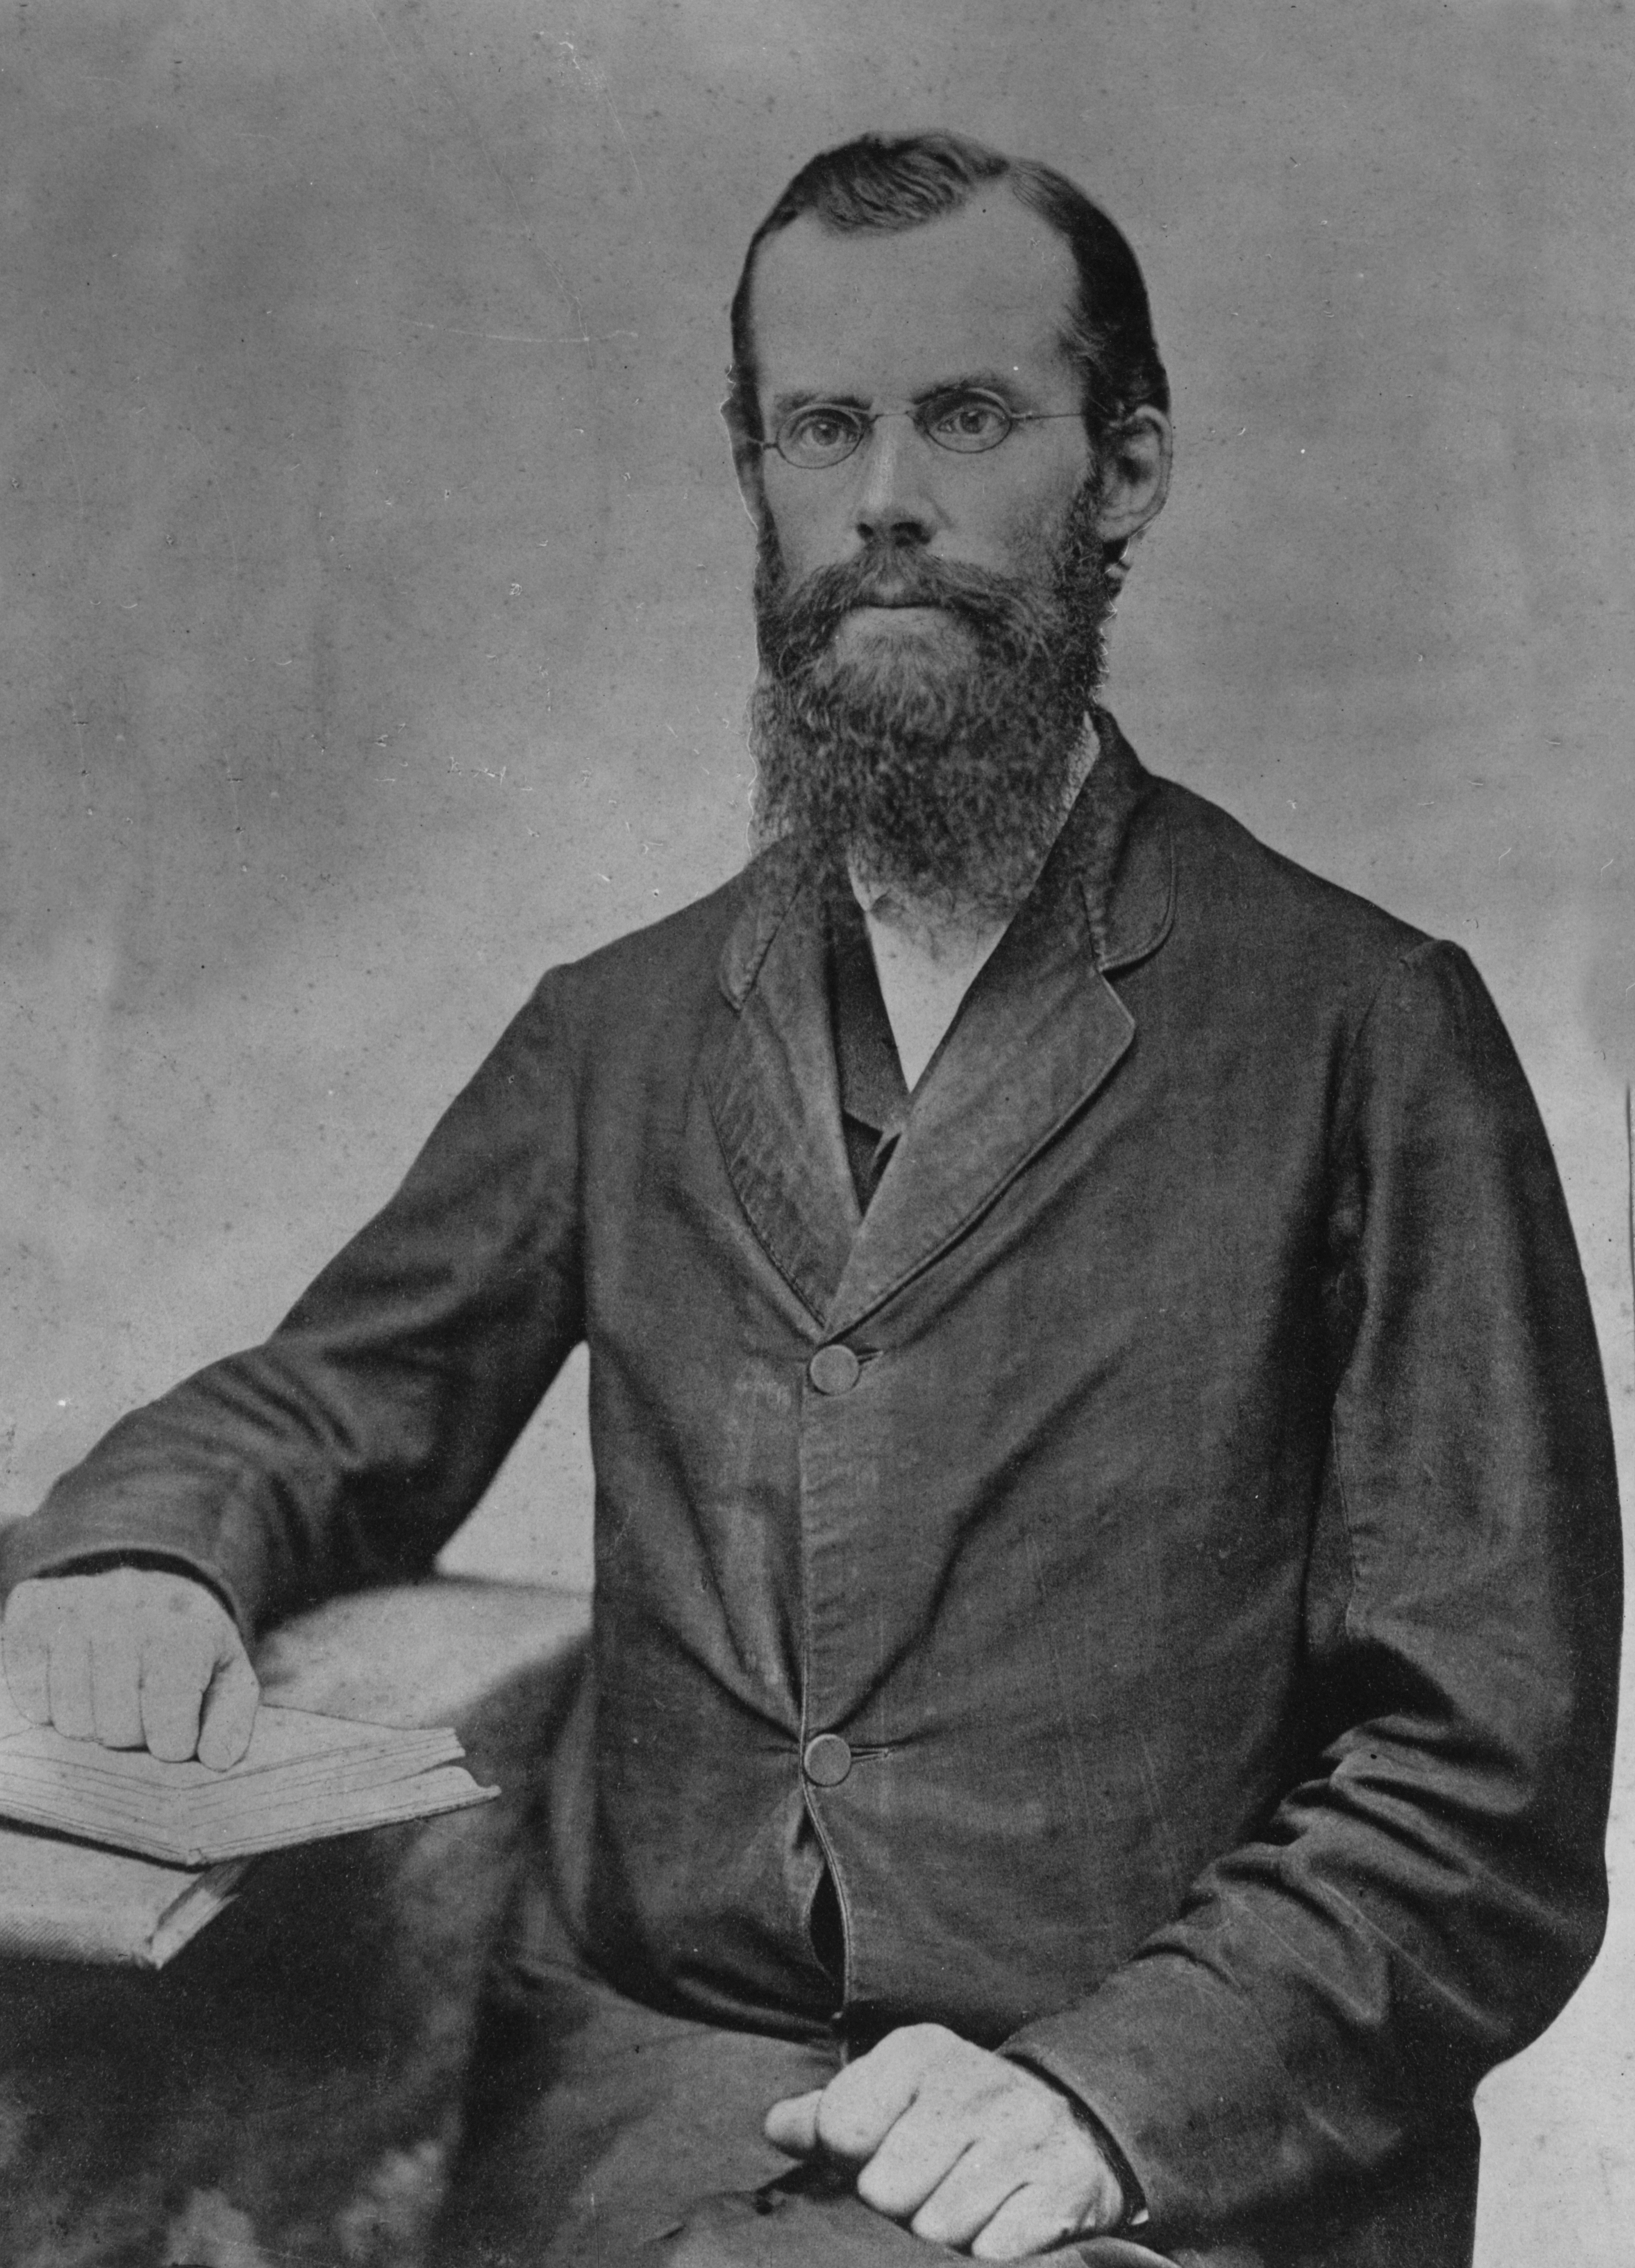
\includegraphics[width=1\linewidth]{images/john-nevins-andrews.jpg}
    \caption*{John Nevins Andrews (1829-1883)}
    \label{fig:j-n-andrews}
\end{figure}


J. N. Andrews said, \others{\textbf{The doctrine of the Trinity which was established in the church by the council of Nicea, A. D. 325}. \textbf{This doctrine \underline{destroys the personality of God, and his Son Jesus Christ our Lord}}...}[John. N. Andrews, The Advent Review and Sabbath Herald, March 6, 1855, p. 185][http://documents.adventistarchives.org/Periodicals/RH/RH18550306-V06-24.pdf]


J. N. Andrews a spus, \others{\textbf{Doctrina Trinității care a fost stabilită în biserică de conciliul de la Niceea, 325 d.Hr.}. \textbf{Această doctrină \underline{distruge personalitatea lui Dumnezeu și a Fiului Său Isus Hristos, Domnul nostru}}...}[John. N. Andrews, The Advent Review and Sabbath Herald, 6 martie 1855, p. 185][http://documents.adventistarchives.org/Periodicals/RH/RH18550306-V06-24.pdf]


In the context of the trinitarian understanding of the \emcap{personality of God}, it is safe to say that the \emcap{personality of God}, or the quality or state of God being a person, in any understanding of Trinity doctrine is a mystery. The problem is that there is no clear view of who is that \textit{one God} who is a person? The underlying claim is made that God is One yet Three, or One in Three; yes, God is a person, and He is one, yet simultaneously He is three persons. This view can never hold any clear perception of the \emcap{personality of God}. Also, it will deny the clearest testimony of the Scriptures that the one God is the Father, and that Christ is truly His only begotten Son. Most trinitarian brothers would agree that Christ is a real and definite being but if a trinitarian were to accept the Father as a real and definite Being, he would also need to accept the Holy Spirit as a real and definite being, thus denying the Holy Spirit as being a \textit{spirit}, the means by which the Father and Son are omnipresent. Conversely, if a trinitarian accepted the Holy Spirit to be a literal spirit, having no body nor form, then he would deny the Father to be a real, definite being. In conversation over the quality or state of God being a person, there is never a clear view of the matter with promoters of the Trinity doctrine; it is subterfuge. \textit{‘Subterfuges’} is a word Sister White used to describe the deception by artifice or stratagem in order to conceal, escape, or evade\footnote{\href{https://www.merriam-webster.com/dictionary/subterfuges}{The Merriam-Webster, ‘subterfuges’} - “\textit{deception by artifice or stratagem in order to conceal, escape, or evade}”} the truth; in other words, something that you cannot grab by head or tail. This is the primary reason Sister White did not engage in the Trinity discussion that would come up in the Seventh-day Adventist Church.


În contextul înțelegerii trinitariene a \emcap{personalității lui Dumnezeu}, este sigur să spunem că \emcap{personalitatea lui Dumnezeu}, sau caracteristica sau starea prin care Dumnezeu este definit ca persoană, în orice înțelegere a doctrinei Trinității este un mister. Problema este că nu există o viziune clară despre cine este acel \textit{Dumnezeu unic} care este o persoană? Afirmația de bază care se face este că Dumnezeu este Unul și totuși Trei, sau Unul în Trei; da, Dumnezeu este o persoană, și El este unul, și totuși simultan El este trei persoane. Această viziune nu poate avea niciodată o percepție clară asupra \emcap{personalității lui Dumnezeu}. De asemenea, va nega cea mai clară mărturie a Scripturilor că singurul Dumnezeu este Tatăl și că Hristos este cu adevărat singurul Său Fiu născut. Majoritatea fraților trinitarieni ar fi de acord că Hristos este o ființă reală și definită, dar dacă un trinitarian ar accepta pe Tatăl ca o Ființă reală și definită, ar trebui de asemenea să accepte pe Duhul Sfânt ca o ființă reală și definită, negând astfel Duhul Sfânt ca fiind un \textit{duh}, mijlocul prin care Tatăl și Fiul sunt omniprezenți. Invers, dacă un trinitarian ar accepta că Duhul Sfânt este un duh literal, neavând nici corp, nici formă, atunci ar nega că Tatăl este o ființă reală, definită. În conversația despre caracteristica sau starea prin care Dumnezeu este definit ca persoană, nu există niciodată o viziune clară a problemei cu promotorii doctrinei Trinității; este subterfugiu. \textit{‘Subterfugii’} este un cuvânt pe care Sora White l-a folosit pentru a descrie înșelăciunea prin artificiu sau stratageme pentru a ascunde, scăpa sau evita\footnote{\href{https://www.merriam-webster.com/dictionary/subterfuges}{The Merriam-Webster, ‘subterfuges’} - “\textit{înșelăciune prin artificiu sau stratageme pentru a ascunde, scăpa sau evita}”} adevărul; cu alte cuvinte, ceva ce nu poți prinde nici de cap, nici de coadă. Acesta este motivul principal pentru care Sora White nu s-a angajat în discuția despre Trinitate care urma să apară în Biserica Adventistă de Ziua a Șaptea.


\egw{I was cautioned not to enter into controversy \textbf{regarding the question} that \textbf{\underline{will come up}} over \textbf{these things, because controversy \underline{might lead men to resort to subterfuges, and their minds would be led away from the truth of the Word of God to assumption and guesswork}}. \textbf{The more that fanciful theories are discussed, the \underline{less men will know of God and of the truth that sanctifies the soul}}.}[Lt232-1903.41; 1903][https://egwwritings.org/read?panels=p10197.50]


\egw{Am fost avertizată să nu intru în controversă \textbf{cu privire la întrebarea} care \textbf{\underline{va apărea}} despre \textbf{aceste lucruri, pentru că controversa \underline{ar putea determina oamenii să recurgă la subterfugii, iar mințile lor ar fi îndepărtate de la adevărul Cuvântului lui Dumnezeu spre presupuneri și speculații}}. \textbf{Cu cât sunt discutate mai multe teorii fanteziste, cu \underline{atât mai puțin vor ști oamenii despre Dumnezeu și despre adevărul care sfințește sufletul}}.}[Lt232-1903.41; 1903][https://egwwritings.org/read?panels=p10197.50]


When we read the works of Seventh-day Adventist pioneers on the \emcap{personality of God}, we see that they did not fall into the Trinity trap. Their non-trinitarian views of God were not due to ignorance, but a knowledge of the truth on the \emcap{personality of God}. They were of keen and noble intellect, understanding the thin line between the truth and error. Their understanding of the \emcap{personality of God} is balanced and solid, strongly supported by the plain and simple “\textit{thus says the Lord}”.


Când citim lucrările pionierilor adventiști de ziua a șaptea despre \emcap{personalitatea lui Dumnezeu}, vedem că ei nu au căzut în capcana Trinității. Viziunile lor non-trinitariene despre Dumnezeu nu s-au datorat ignoranței, ci cunoașterii adevărului despre \emcap{personalitatea lui Dumnezeu}. Ei erau de un intelect ascuțit și nobil, înțelegând linia subțire dintre adevăr și eroare. Înțelegerea lor despre \emcap{personalitatea lui Dumnezeu} este echilibrată și solidă, puternic susținută de simplul și clarului “\textit{așa zice Domnul}”.


Many Adventists today accept the Trinity doctrine because Ellen White supposedly accepted it and promoted it. This is far from the truth and such a conclusion is predicated on lacking knowledge of the Spirit of Prophecy. If anyone was acquainted with the beliefs of Sister White, it was her husband James White. Here is what he has to say about the writings of his wife:


Mulți adventiști de astăzi acceptă doctrina Trinității pentru că Ellen White ar fi acceptat-o și promovat-o. Aceasta este departe de adevăr și o astfel de concluzie se bazează pe lipsa cunoașterii Spiritului Profetic. Dacă cineva era familiarizat cu credințele Sorei White, acela era soțul ei, James White. Iată ce are de spus despre scrierile soției sale:


\others{\textbf{We invite all to compare the testimonies of the Holy Spirit through Mrs. W., with the word of God}. \textbf{And in this we do not invite you to compare them \underline{with your creed}}. That is quite another thing. \textbf{\underline{The trinitarian may compare them with his creed, and because they do not agree with it, condemn them}}. The observer of Sunday, or the man who holds eternal torment an important truth, and the minister that sprinkles infants, may each condemn the testimonies’ of Mrs. W. because they do not agree with their peculiar views. And a hundred more, each holding different views, may come to the same conclusion. \textbf{But their genuineness can never be tested in this way}.}[James S. White, The Advent Review, and Herald of the Sabbath, June 13, 1871][https://documents.adventistarchives.org/Periodicals/RH/RH18710613-V37-26.pdf]


\others{\textbf{Invităm pe toți să compare mărturiile Duhului Sfânt prin Dna W., cu cuvântul lui Dumnezeu}. \textbf{Și în aceasta nu vă invităm să le comparați \underline{cu crezul vostru}}. Aceasta este cu totul altceva. \textbf{\underline{Trinitarianul poate să le compare cu crezul său și, pentru că nu sunt de acord cu el, să le condamne}}. Păzitorul duminicii, sau omul care consideră chinul veșnic un adevăr important, și pastorul care stropește copiii, fiecare poate condamna mărturiile Dnei W. pentru că nu sunt de acord cu viziunile lor particulare. Și o sută de alții, fiecare având viziuni diferite, pot ajunge la aceeași concluzie. \textbf{Dar autenticitatea lor nu poate fi niciodată testată în acest fel}.}[James S. White, The Advent Review, and Herald of the Sabbath, 13 iunie 1871][https://documents.adventistarchives.org/Periodicals/RH/RH18710613-V37-26.pdf]


James White was the closest associate of Ellen White, the person who was one with her in God’s uplifting of the Seventh-day Adventist Church. We have a clear and direct testimony from him that Ellen White’s writings are not trinitarian. Today, scholars put a false narrative that Ellen White grew in her understanding of the Trinity doctrine, and eventually accepted and preached it. But we see that Ellen White did not change her standpoint on the \emcap{personality of God} nor did she adhere to the Trinity doctrine. She was unambiguous in her claim that she never did. When the Kellogg crisis came over the \emcap{personality of God}, she remained firm in her view, just as all early Seventh-day Adventist pioneers did—and her dealings with Dr. Kellogg prove that. It is true, the Trinity doctrine \textit{cannot be accepted by those who are loyal to the faith and to the principles that have withstood all the opposition of satanic influences}.\footnote{\egw{Patchwork theories cannot be accepted by those who are loyal to the faith and to the principles that have withstood all the opposition of satanic influences}[Lt253-1903.28; 1903][https://egwwritings.org/read?panels=p14068.9980036]} Today’s official narrative that Ellen White was teaching the Trinity echoes Dr. Kellogg’s claim that the Living Temple taught the same thing as Ellen White. \egwinline{\textbf{But God forbid that this sentiment should prevail}.}[SpTB02 53.3; 1904][https://egwwritings.org/read?panels=p417.272]


James White a fost cel mai apropiat asociat al lui Ellen White, persoana care era una cu ea în înălțarea de către Dumnezeu a Bisericii Adventiste de Ziua a Șaptea. Avem o mărturie clară și directă de la el că scrierile lui Ellen White nu sunt trinitariene. Astăzi, învățații pun o narațiune falsă că Ellen White a crescut în înțelegerea ei despre doctrina Trinității și în cele din urmă a acceptat-o și a predicat-o. Dar vedem că Ellen White nu și-a schimbat punctul de vedere despre \emcap{personalitatea lui Dumnezeu} și nici nu a aderat la doctrina Trinității. Ea a fost lipsită de ambiguitate în afirmația ei că nu a făcut-o niciodată. Când a venit criza Kellogg asupra \emcap{personalității lui Dumnezeu}, ea a rămas fermă în viziunea ei, la fel cum au făcut toți pionierii adventiști de ziua a șaptea timpurii—și relațiile ei cu Dr. Kellogg dovedesc acest lucru. Este adevărat, doctrina Trinității \textit{nu poate fi acceptată de cei care sunt loiali credinței și principiilor care au rezistat tuturor opoziției influențelor satanice}.\footnote{\egw{Teoriile de peticire nu pot fi acceptate de cei care sunt loiali credinței și principiilor care au rezistat tuturor opoziției influențelor satanice}[Lt253-1903.28; 1903][https://egwwritings.org/read?panels=p14068.9980036]} Narațiunea oficială de astăzi că Ellen White învăța Trinitatea face ecou afirmației Dr. Kellogg că Templul viu învăța același lucru ca Ellen White. \egwinline{\textbf{Dar ferească Dumnezeu ca această opinie să prevaleze}.}[SpTB02 53.3; 1904][https://egwwritings.org/read?panels=p417.272]


% Adventist pioneers and the Trinity doctrine

\begin{titledpoem}
    \stanza{
        The pioneers stood firm against the Trinity's sway, \\
        Their testimony clear as the light of day. \\
        They saw how this doctrine did subtly disguise, \\
        What Scripture reveals to discerning eyes.
    }

    \stanza{
        James White declared it among "popular fables" found, \\
        A teaching that makes God's personality unsound. \\
        For Father and Son as distinct beings stand, \\
        Not merged into one as the Trinity planned.
    }

    \stanza{
        Two separate persons with purpose aligned, \\
        In spirit and action, united in mind. \\
        Just as disciples in Christ become one, \\
        Yet remain individual under God's Son.
    }

    \stanza{
        The Holy Spirit, God's presence divine, \\
        Not a separate being of the Godhead's design. \\
        But truly God's Spirit sent forth from above, \\
        The Father's representative, agent of love.
    }

    \stanza{
        No Scripture supports what tradition declared, \\
        When at Nicea this doctrine was shared. \\
        John seventeen shatters the trinitarian view, \\
        Revealing the Father and Son as beings true.
    }

    \stanza{
        Christ's divinity rests not in mysterious three, \\
        But in His begotten Sonship we see. \\
        The express image of His Father's face, \\
        Inheriting fullness of divine grace.
    }

    \stanza{
        The pioneers knew what the Bible made clear, \\
        That God is the Father, a Being most dear. \\
        A personal, spiritual presence on high, \\
        Omnipresent through Spirit, yet dwelling on high.
    }

    \stanza{
        So stands the truth against error's long night, \\
        Preserved by the pioneers and Sister White. \\
        Not through confusion or mystical thought, \\
        But through plain Scripture the truth has been taught.
    }
\end{titledpoem}